\subsection{Replication}

In the current section, we will first compare the results of our replication study with the results of \cite{Sulpizio_McQueen_2012}'s real word eye-tracking task. \cite{Sulpizio_McQueen_2012}'s study focused on answering three questions. 1) To what extent do target vs competitor fixations differ in the process of word recognition for tri-syllabic Italian words that differ in stress? 2) Is there a bias in fixation patterns due to distributional inequalities in frequency of penultimate and antepenultimate? 3) To what extent do acoustic cues affect word recognition in trisyllabic word recognition for stress contrastive words? 

After these analyses, we run additional analyses on the first and third research questions to tease apart the role of individual differences in both simple word recognition and how these individual differences affect cue integration across word recognition for contrastive stress patterns. 

\subsubsection{Acoustic analysis}
Results of acoustic analysis can be found in Table \ref{tab:acoustics}. Exactly like \cite{Sulpizio_McQueen_2012}, all measures we significantly different between syllables besides spectral tilt in penultimate words. In penultimate words, first syllables were louder, higher, and shorter. In contrast, for antepenultimate words, the first syllables was louder, higher, longer, with great spectral tilt.


\subsubsection{Target and competitor analysis}

Here, we attempt to simplify the modeling approach. \cite{Sulpizio_McQueen_2012} did six separate mixed-effects analyses, three on each stress type. The three mixed-effects analyses on each stress type were done on three additive time windows. Instead, we use one large model to capture the effects and use stress type as a predictor that could interact with looks over time. \cite{Sulpizio_McQueen_2012}'s method of separating the data into penultimate and antepenultimate data before analysis allows one to examine if looks increase independently in both stress types (penultimate and antepenultimate). However, the separation of these analyses makes it impossible to know if there is a difference between fixations during the process of word recognition for the two stress patterns. \cite{Sulpizio_McQueen_2012} did not find differences in their separate models. In this way, our modeling approach should capture a difference between stress types if there is one. Another additional difference is the way that we define time windows of interest. In the original study, there were three time periods, one for each stress pattern: penultimate (200-396 ms, 200-566 ms, 200-699 ms) and antepenultimate (200-499 ms, 200-566 ms, 200-669 ms). These time windows correspond to the first syllable, first 1.5 syllables, and the second syllable. Like the original study, we have three time windows but our analyses separate these into three discrete time windows over the first two syllables of the word that are not additive. Additionally, we add a fourth time window to use as baseline looks over the 0-200 ms time window before the participants have time to process the word. That is, we have the first syllable and second syllable as well as a 1.5 window (the average of the first syllable plus half of the second syllable), and the second syllable time window. We did our modeling by starting with a maximal GLMM model defined by predicting binary looks \citep{Barr_2008}. For predictors, we used stress, syllable, visual stimuli (target, competitor, distractors), and their interactions. We used the competitor as baseline to compare looks to targets and distractors so that we could tease apart possible differences between looks in different stress types. We also used the 0-200 ms time window as baseline. Finally, we gave each participant random intercepts.

Model reduction was done by removing the interactions between each respective term and comparing more complex models with simpler models with ANOVA, AIC, and BIC comparison. Through this process, it was found that the parsimonious model (eye-fixations ~ stress + visual stimuli * syllable + (1 | participant.private.id)) provided the best balance of fit and simplicity. This model had the lowest AIC and BIC values among all models tested, indicating a better fit relative to its complexity. Additionally, ANOVA comparisons between the models demonstrated that model 3 was significantly better than simpler models while being sufficiently parsimonious compared to more complex ones.

Results from the target-competitor GLMM found significant effects for several main effects and their interactions. In terms of visual stimuli effects, distractor 1 ($\beta$ = -0.16, \textit{SE} = 0.04, \textit{z} = -4.41, \textit{p} $<$ .001) and target ($\beta$ = -0.17, \textit{SE} = 0.04, \textit{z} = -4.56, \textit{p} $<$ .001) both had significant differences from competitor looks overall suggesting fewer looks to distractors and targets overall. 

Several significant effects were also found across syllables, syllable 1 ($\beta$ = 0.10, \textit{SE} = 0.04, \textit{z} = 2.68, \textit{p} $<$ .01) looks significantly increased as compared to the 0-200 ms time window. Additionally, the interactions between looks to the distractor 1 and syllable 1 ($\beta$ = -0.24, \textit{SE} = 0.05, \textit{z} = -4.71, \textit{p} $<$ .001), distractor 1 and syllable 1.5 ($\beta$ = -0.52, \textit{SE} = 0.06, \textit{z} = -8.88, \textit{p} $<$ .001), and the interaction between looks to the distractor 1 and syllable 2 ($\beta$ = -0.30, \textit{SE} = 0.06, \textit{z} = -5.18, \textit{p} $<$ .001) indicate increasingly less looks to distractors as compared to competitors during syllables 1, 1.5, and 2. Whereas the interactions between looks to the target and syllable 1 ($\beta$ = 0.11, \textit{SE} = 0.05, \textit{z} = 2.08, \textit{p} $<$ .05), looks to target and syllable 1.5 ($\beta$ = 0.55, \textit{SE} = 0.05, \textit{z} = 10.08, \textit{p} $<$ .001), and looks to the target and syllable 2 ($\beta$ = 0.68, \textit{SE} = 0.05, \textit{z} = 12.42, \textit{p} $<$ .001) indicate that looks to target were significantly more than to competitor during syllable 1, 1.5, and even more so in syllable 2. These findings highlight the time course of word recognition over the period of the word. While it would be inappropriate to interpret a NULL effect for stress type, it is worth noting that stress did not come up significant in the models. That is, any additional variance explained by stress and its interactions was found to be unjustified when accounting for added complexity. Proportion of looks to targets, competitors, and distractors over the time course of penultimate and antepenultimate words can be seen in Figure \ref{fig:raw_pen_vs_anti}.

\begin{figure}[H]
  \centering
  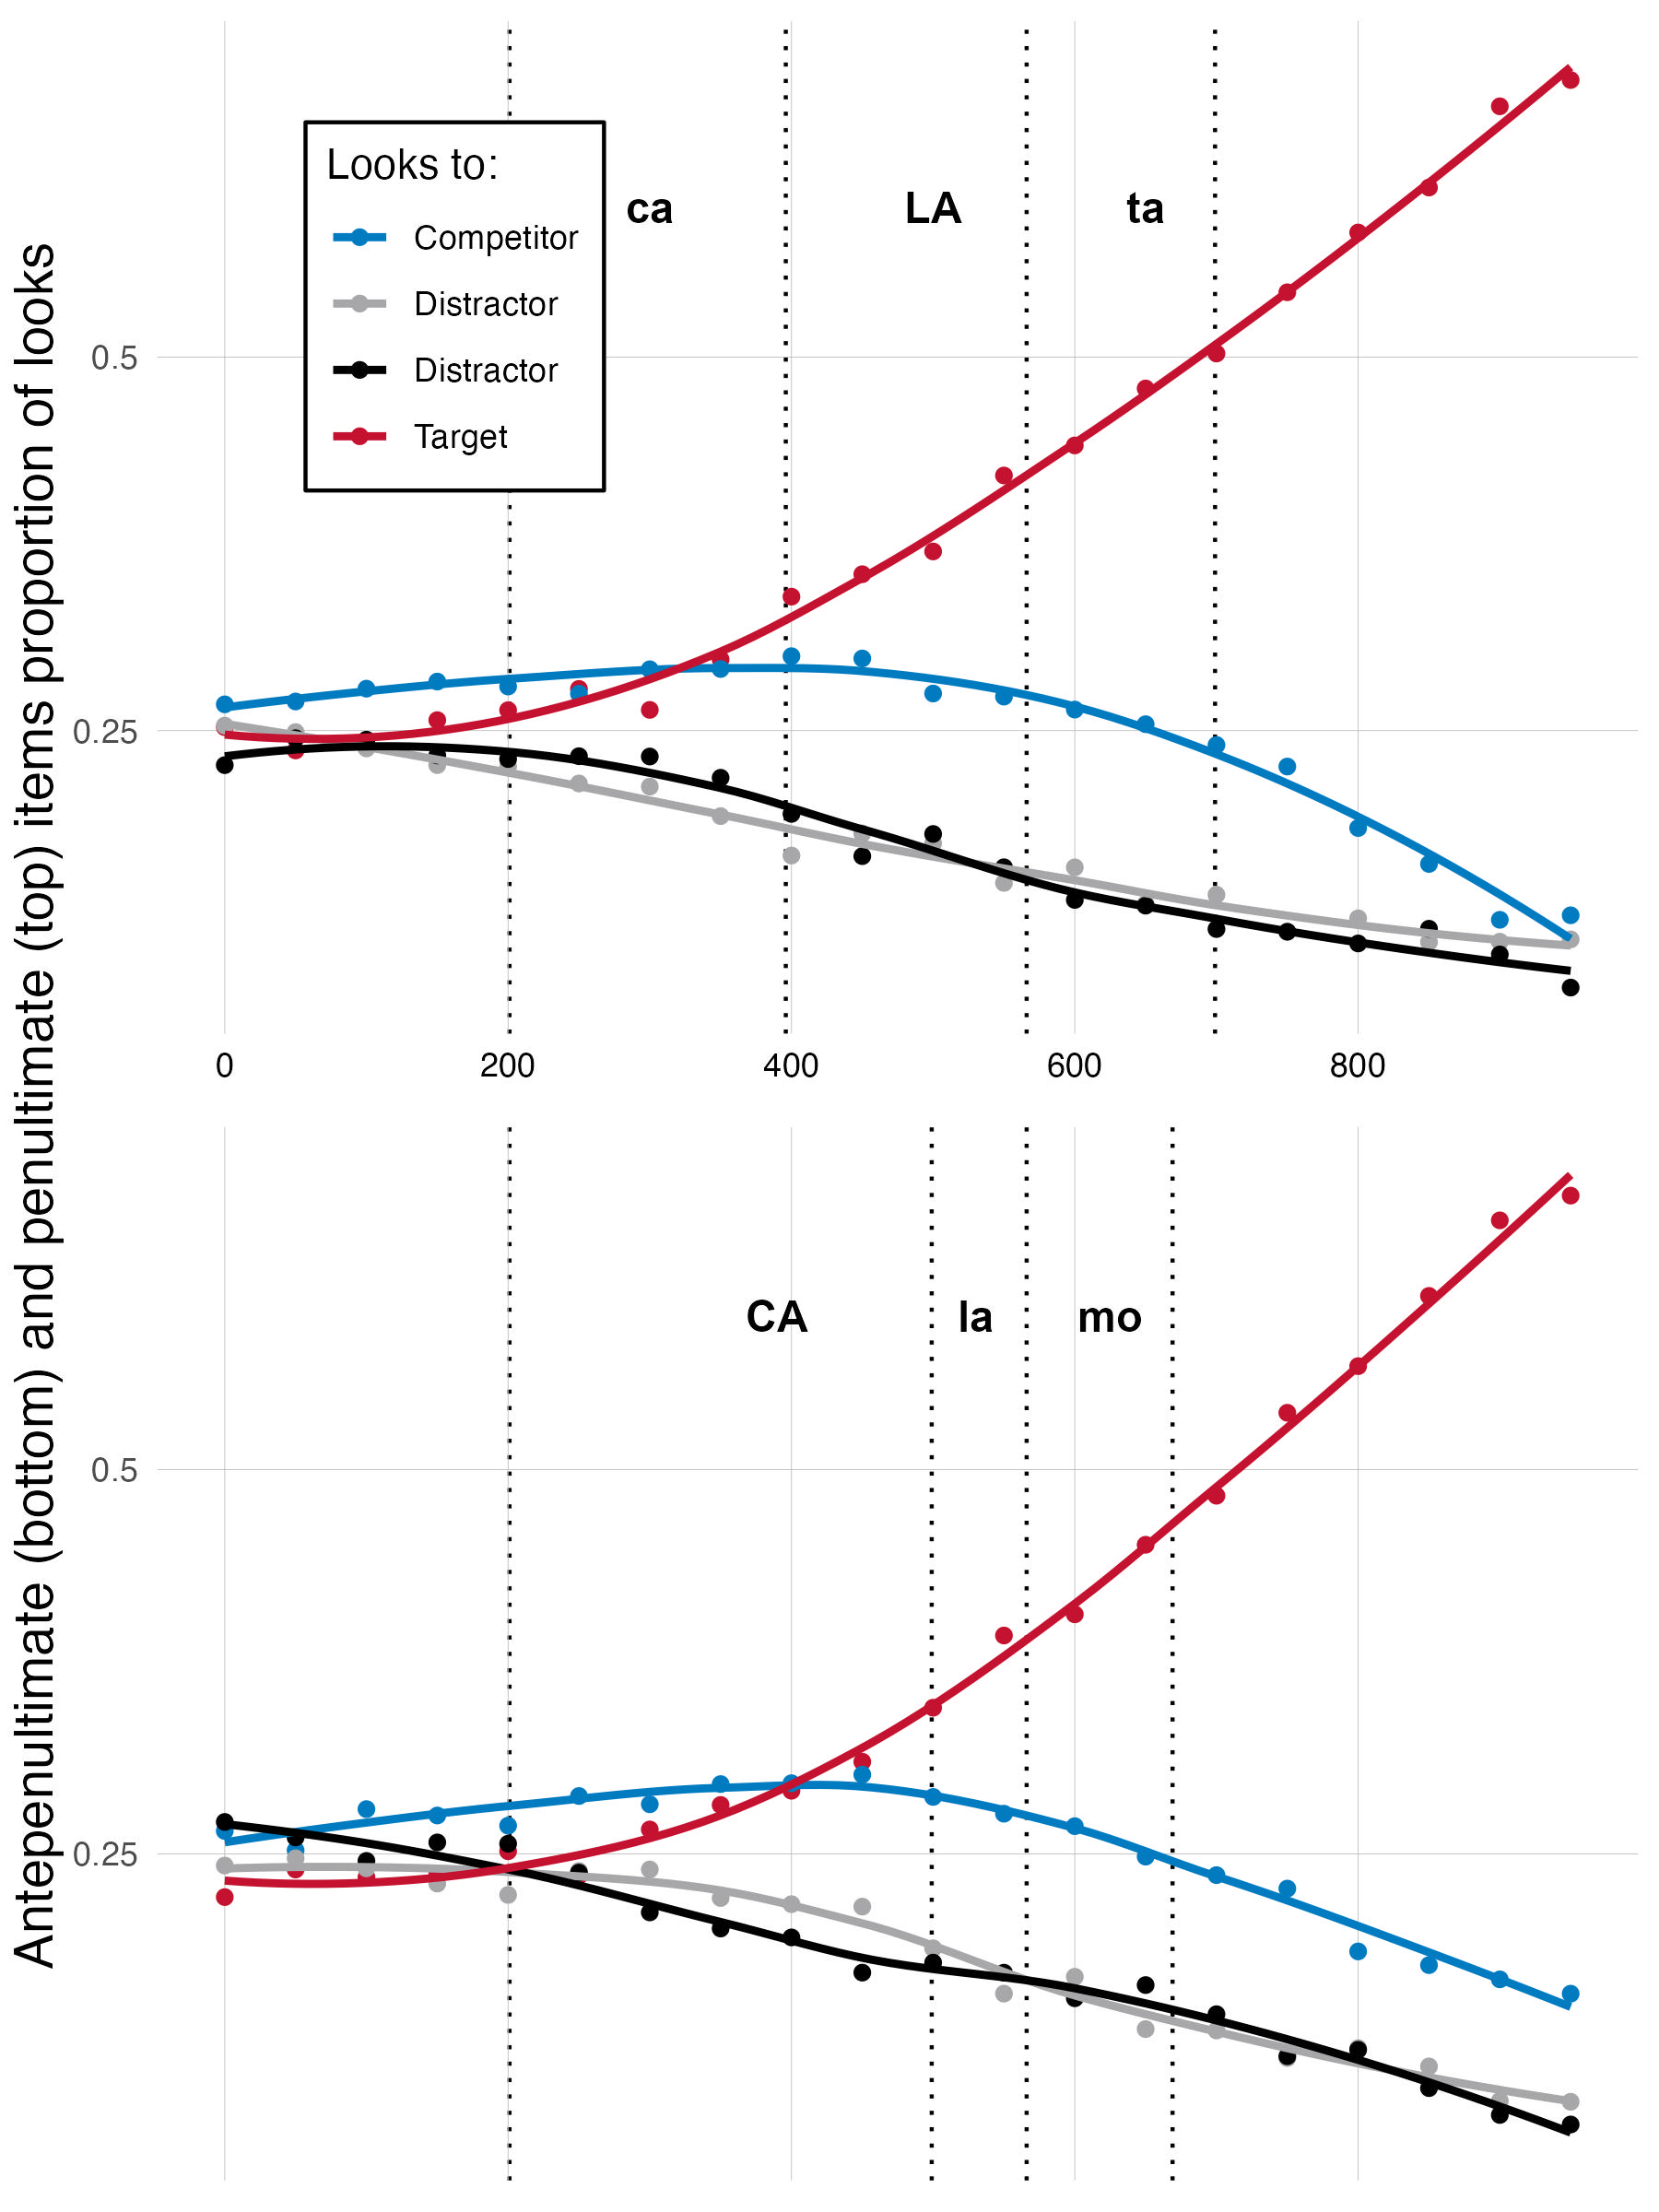
\includegraphics[width=0.6\linewidth]{visuals/pen_vs_anti_pen.jpeg} % Adjust the width as needed
  \caption{Antepenultimate and penultimate competition: The example words Calata (penultimate) and Calamo (antepenultimate) are used to show where syllables begin and end by stress type.}
  \label{fig:raw_pen_vs_anti}
\end{figure}

\subsubsection{Target bias analysis}

Due to the distributional bias that is inherent in Italian stress patterns \cite{Sulpizio_McQueen_2012}, a linear mixed-effects model was fit on proportions of looks to target values only. That is, we are interested in examining if there is a bias in target looks as a proportion to the total captured fixations across stress types. To do this we predicted mean looks to targets with stress (baseline - antepenultimate) and syllable (1.5 and 2 - baseline 2) to ensure that there was no bias overall in looks by stress type over the word. We additionally used word as a random intercept. Like \cite{Sulpizio_McQueen_2012}, our models found no bias in looks to targets over either stress at any syllable. No significant results were found.   


\subsubsection{Cue integration}

In this section, we investigate how different speech cues influence eye-fixation during the process of word recognition. To do this, we built four mixed-effects models, two of which explored within stress type at syllable 1 and 2. For both penultimate and antepenultimate models, target looks were used as the dependent variable. The cue of the respective syllables were then used to predict looks to target. The model structure for all four of the models is identical. That is, target looks were predicted by four scaled measurements of the auditory stimuli (mean pitch, mean amplitude, tilt, and duration) and all possible two-way interactions. Additionally, word is used as a random intercept as well. All models started with maximal models and were reduced using a backward stepwise selection procedure. 

The backward stepwise selection procedure began with the full model, which included all main effects and their interactions. Non-significant interactions were removed step-by-step, starting with the highest-order interactions, based on the significance levels obtained from Wald z-tests. Each step involved refitting the model without the least significant interaction or main effect and comparing the fit of the reduced model to the previous model using the AIC. The process continued until the removal of any additional terms resulted in a significant increase in the AIC, indicating a poorer fit to the data. This method ensures that the final models are parsimonious, retaining only those predictors that contribute significantly to explaining the variance in target looks. While \cite{Sulpizio_McQueen_2012} confirmed analyses with reverse regression, their primary analysis focused on correlations between variables. Our analyses also include interactions between speech cues which may allow us to capture more subtle variation across fixations for Italian word stress.

For the penultimate syllable 1 model, like \cite{Sulpizio_McQueen_2012}, no main effects were significant. However, the interaction between tilt and pitch ($\delta = -0.26$, \textit{SE} = 0.10, \textit{z} = -2.61, $p < 0.01$) suggests fewer looks to targets with higher tilt and pitch. Further, the interaction between pitch and duration ($\delta = 0.20$, \textit{SE} = 0.06, \textit{z} = 3.13, $p < 0.01$) indicates more looks to targets with higher pitch and longer duration stimuli.

For the antepenultimate syllable 1 model, main effects include pitch results ($\delta = -0.21$, \textit{SE} = 0.07, \textit{z} = -3.01, $p < 0.01$), which indicate that higher pitch words lead to fewer looks to targets for antepenultimate words. Additionally, several two-way interactions were found. The interaction between pitch and amplitude ($\delta = 0.20$, \textit{SE} = 0.08, \textit{z} = 2.39, $p < 0.05$) indicates more looks to targets with higher pitch and amplitude stimuli. Similarly, the interaction between pitch and duration ($\delta = 0.20$, \textit{SE} = 0.07, \textit{z} = 2.62, $p < 0.01$) suggests more looks to targets with higher pitch and longer duration. 

Starting with the main effects for the penultimate second syllable model, unlike \cite{Sulpizio_McQueen_2012}, amplitude results ($\delta = 0.66$, \textit{SE} = 0.21, \textit{z} = 3.13, $p < 0.01$) indicate that higher amplitude leads to more looks to targets during the second syllable. Duration results ($\delta = -0.30$, \textit{SE} = 0.12, \textit{z} = -2.53, $p < 0.05$) indicate that longer duration leads to fewer looks to targets.

Additionally, several two-way interactions were found. The interaction between amplitude and pitch ($\delta = -0.35$, \textit{SE} = 0.14, \textit{z} = -2.50, $p < 0.05$) indicates fewer looks to targets with higher amplitude and pitch. The interaction between tilt and pitch ($\delta = 0.20$, \textit{SE} = 0.09, \textit{z} = 2.35, $p < 0.05$) indicates more looks to targets with higher tilt and pitch. The interaction between duration and pitch ($\delta = 0.26$, \textit{SE} = 0.09, \textit{z} = 2.99, $p < 0.01$) indicates more looks to targets with longer duration and higher pitch. The interaction between amplitude and duration ($\delta = -0.47$, \textit{SE} = 0.16, \textit{z} = -2.96, $p < 0.01$) indicates fewer looks to targets with higher amplitude and longer duration.

In the antepenultimate second syllable model, pitch results ($\delta = -2.09$, \textit{SE} = 0.60, \textit{z} = -3.48, $p < 0.001$) indicate that higher pitch leads to fewer looks to targets. Duration results ($\delta = -1.25$, \textit{SE} = 0.48, \textit{z} = -2.58, $p < 0.01$) suggest that longer duration leads to fewer looks to targets.

Lastly, the interaction between pitch and duration ($\delta = -1.60$, \textit{SE} = 0.61, \textit{z} = -2.62, $p < 0.01$) indicates fewer looks to targets with higher pitch and longer duration.

\begin{figure}[H]
  \centering
  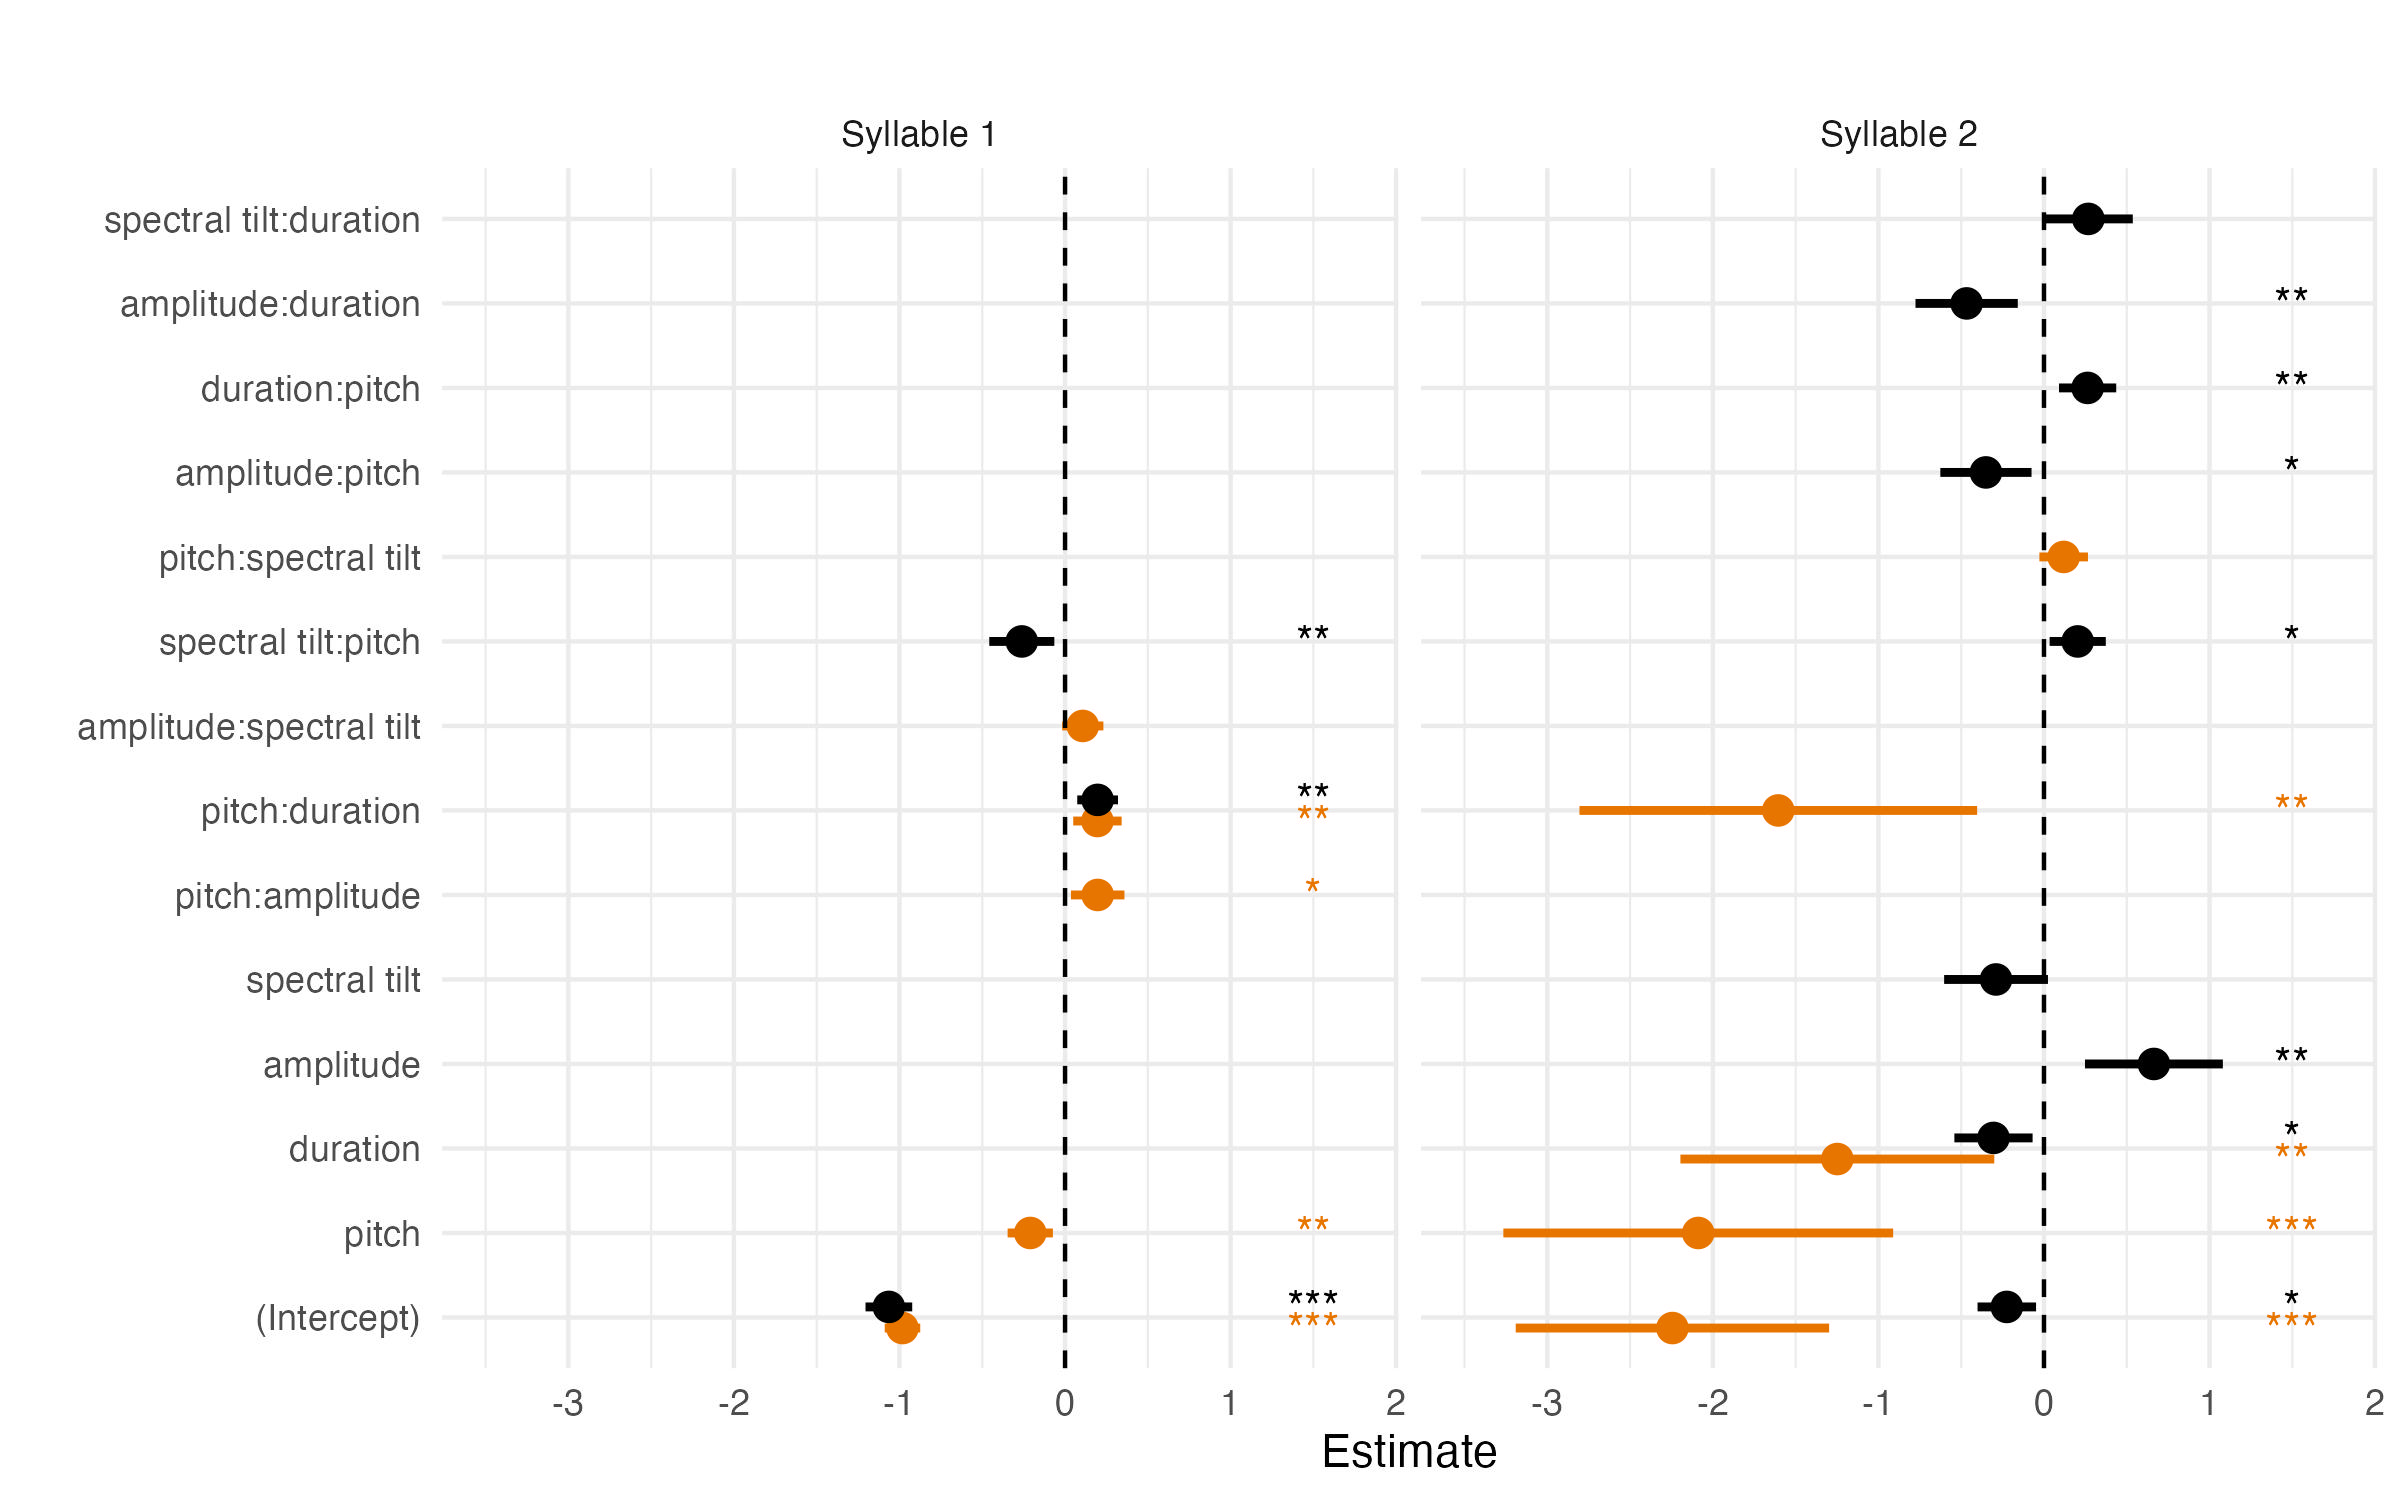
\includegraphics[width=1\linewidth]{visuals/analysis_3_plot.jpeg} % Adjust the width as needed
  \caption{Model selection outcomes for penultimate and antepenultimate cue models for first and second syllable.}
  \label{fig:analysis_3_plot }
\end{figure}

\subsection{Extension}

In this section, we extend the replication by incorporating additional cognitive measures to understand their influence on word recognition. The measures include various auditory processing skills (pitch d', duration d', rise time d', formant d'), English and Italian language proficiency (measured by the Lextale tasks), and autism spectrum traits (ASDQ). The primary aim is to identify which of these measures significantly contribute to target looks during word recognition and how they interact with Italian stress patterns over the first two segmentally identical syllable positions. We employed LASSO (Least Absolute Shrinkage and Selection Operator) regression to perform variable selection due to its ability to handle high-dimensional data and multi-collinearity \citep{Zhang2020, Tibshirani1996}. Early data exploration revealed high correlations between the four battery tasks. LASSO helps resolve this by penalizing the absolute size of the regression coefficients. This allows for the identification of the most relevant predictors. The LASSO regression was applied separately for each stress pattern. Centered and regularized individual differences scores can be found in Figure \ref{fig:plot_raw_task}.


\begin{figure}[H]
  \centering
  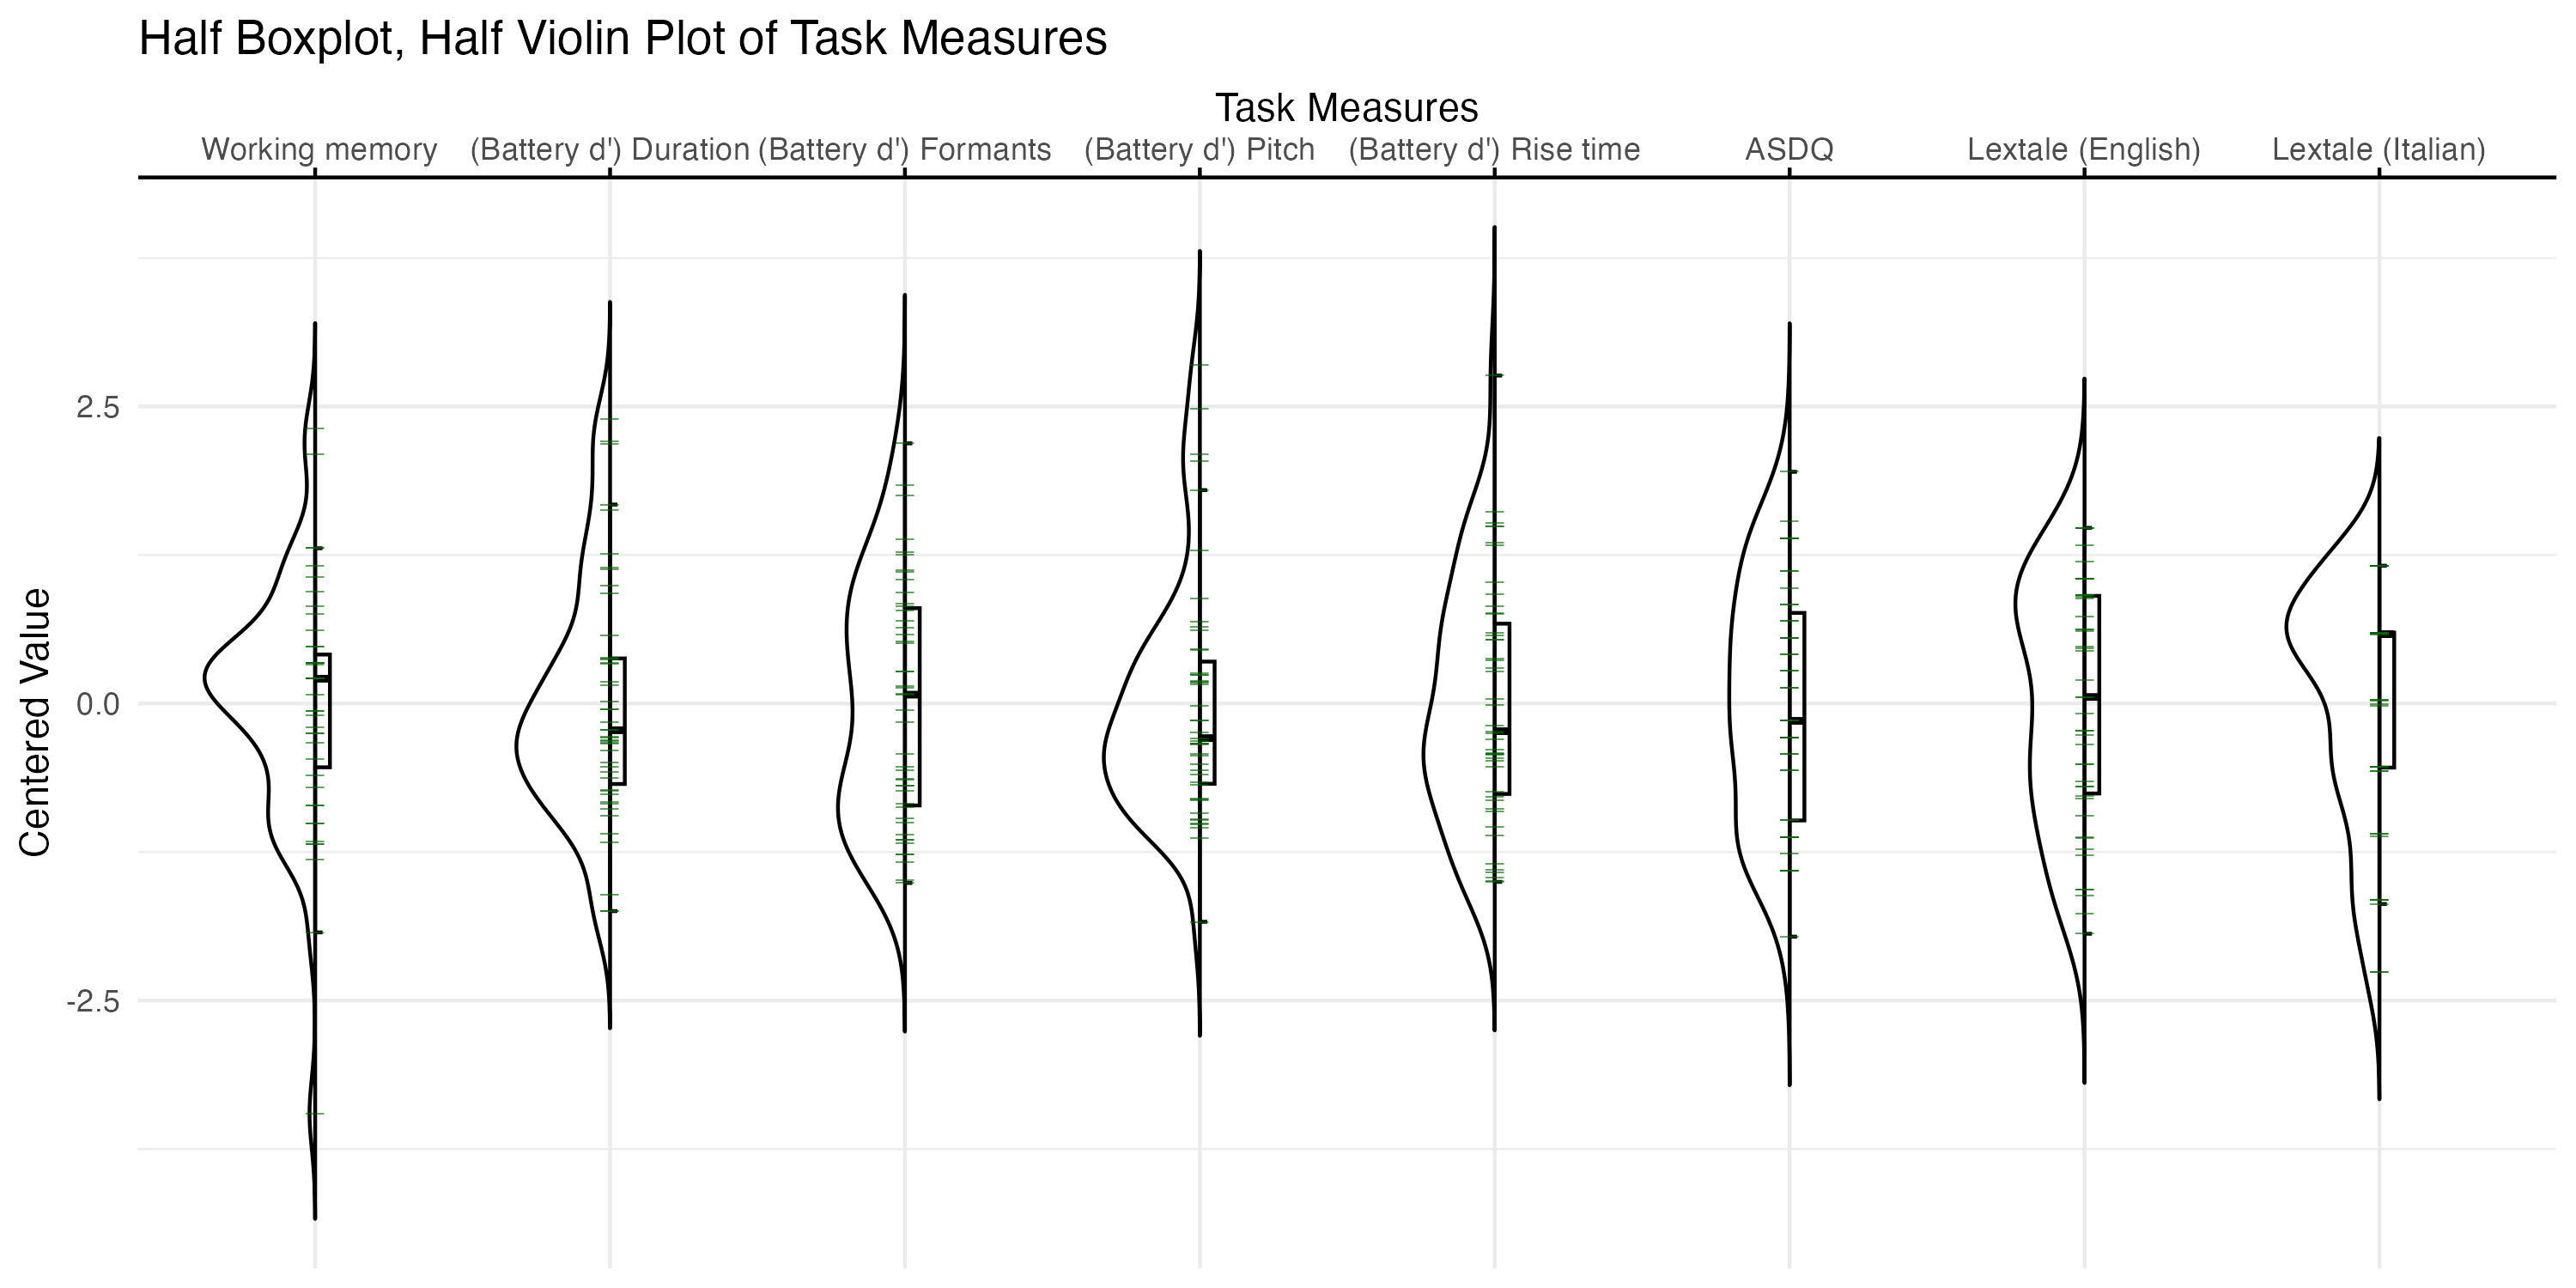
\includegraphics[width=1\linewidth]{visuals/plot_raw_task.jpeg} % Adjust the width as needed
  \caption{Antepenultimate and penultimate model}
  \label{fig:plot_raw_task}
\end{figure}


The significant predictors and their interactions were identified using LASSO regression, and the resulting variables were used to fit a Generalized Linear Mixed Model (GLMM). The GLMMs provide detailed insights into how each predictor affects target looks, accounting for random intercepts by word.


\subsubsection{Target and competitor analysis - individual differences}

Before fitting the models, a LASSO regression was performed to select significant variables. The LASSO model was fit using a $\lambda$ search space. Cross-validation was employed to find the best $\lambda$. Significant variables based on LASSO coefficients were selected and used to construct the formula for the GLMMs.

\textit{Extended penultimate stress analysis}. 

In the penultimate stress model, the formula included duration d', English Lextale, Italian Lextale, and their interactions with syllable and ASDQ. 

Significant findings include a negative effect of duration d' ($\delta = -0.56$, \textit{SE} = 0.22, \textit{z} = -2.50, $p < 0.05$) and a positive effect of Italian Lextale score ($\delta = 2.54$, \textit{SE} = 1.14, \textit{z} = 2.23, $p < 0.05$), indicating that duration sensitivity has a negative effect on target fixations while the Italian Lextale has a positive effect. Interactions between English Lextale and syllable 1 ($\delta = 0.54$, \textit{SE} = 0.22, \textit{z} = 2.50, $p < 0.05$), syllable 1.5 ($\delta = 0.82$, \textit{SE} = 0.20, \textit{z} = 4.17, $p < 0.001$), and syllable 2 ($\delta = 0.91$, \textit{SE} = 0.21, \textit{z} = 4.38, $p < 0.001$) indicate more looks to targets with higher English Lextale scores increasing over syllables.

\textit{Extended antepenultimate stress analysis}.

In the antepenultimate stress model, the formula included pitch d', English Lextale, Italian Lextale, and their interactions with syllable and duration d'. 

Significant findings include a positive effect of pitch d' ($\delta = 0.58$, \textit{SE} = 0.13, \textit{z} = 4.31, $p < 0.001$), English Lextale ($\delta = 0.57$, \textit{SE} = 0.20, \textit{z} = 2.84, $p < 0.01$), and Italian Lextale ($\delta = 3.08$, \textit{SE} = 1.09, \textit{z} = 2.84, $p < 0.01$), indicating that pitch discrimination ability, English proficiency, and Italian word knowledge are all predictive of more target looks. Interactions between duration d' and syllable 1 ($\delta = -1.37$, \textit{SE} = 0.38, \textit{z} = -3.66, $p < 0.001$), duration d' and syllable 1.5 ($\delta = -1.85$, \textit{SE} = 0.58, \textit{z} = -3.22, $p < 0.01$), and duration d' and syllable 2 ($\delta = -1.84$, \textit{SE} = 0.47, \textit{z} = -3.95, $p < 0.001$) indicate fewer looks to targets with higher duration d' over syllables. Additionally, the interactions between English Lextale and syllable 1 ($\delta = 0.26$, \textit{SE} = 0.12, \textit{z} = 2.22, $p < 0.05$), syllable 1.5 ($\delta = 0.74$, \textit{SE} = 0.15, \textit{z} = 5.01, $p < 0.001$), and syllable 2 ($\delta = 0.70$, \textit{SE} = 0.13, \textit{z} = 5.39, $p < 0.001$) indicate more looks to targets with higher English Lextale for these syllables. 

\subsubsection{Cue integration - individual differences}

Like the extended analysis for simple word recognition. For cue integration and individual differences, we use a LASSO regression to select significant variables before fitting GLMMs. In the model selection process for fitting the generalized linear mixed models (GLMM), we then create the design matrix and response vector using a set of predictor variables, which include working memory, duration d', pitch d', risetime d', formants d', English Lextale, Italian Lextale, ASDQ and their interactions with syllable-pitch, syllable-duration, syllable-amplitude, and syllable-spectral tilt. To identify the most relevant predictors, we employ LASSO regression in the same manner as the above analysis. Like the above model, we use the significant variables identified by the LASSO regression, to construct a formula for the GLMM, which includes a random effect for the word. 

For the penultimate syllable 1 extended model, the final model included risetime d', ASDQ, syllable-pitch, duration, and their interactions with scaled acoustic measures. No predictors or interactions had significant effects.

For the antepenultimate syllable 1 model, the formula included duration d', pitch d', English Lextale, Italian Lextale, and their interactions with syllable-duration and syllable-spectral tilt. Significant findings included a positive effect of pitch d' (Estimate = 1.02, \textit{SE} = 0.22, \textit{z} = 4.58, \textit{p} $<$ 0.001) indicating more looks to targets for higher pitch words during syllable 1 processing. The English Lextale was also significant (Estimate = 1.00, \textit{SE} = 0.32, \textit{z} = 3.16, \textit{p} $<$ .01), indicating that higher English proficiency predicts more antepenultimate target fixations during syllable 1. The Italian Lextale was also significant (Estimate = 4.78, \textit{SE} = 1.92, \textit{z} = 2.50, \textit{p} $<$ .05), while the interaction between duration d' and syllable-duration (Estimate = -0.87, \textit{SE} = 0.42, \textit{z} = -2.10, \textit{p} $<$ .05) and the interaction between syllable-spectral tilt and risetime d' (Estimate = -0.61, \textit{SE} = 0.30, \textit{z} = -2.05, \textit{p} $<$ .05) indicate less looks to target during syllable 1 for higher duration discrimination ability and word duration as well as less looks to targets for words with higher spectral tilt and for those with better risetime discrimination.

For the penultimate syllable 2 model, variables included formats d', English Lextale, ASDQ, Italian Lextale, and their interactions with syllable-pitch, syllable-amplitude, and syllable-duration. Significant findings included a positive effect of English Lextale (Estimate = 0.90, \textit{SE} = 0.38, \textit{z} = 2.40, \textit{p} $<$ .05), Italian Lextale (Estimate = 8.58, \textit{SE} = 2.49, \textit{z} = 3.45, \textit{p} $<$ 0.001), and a negative interaction between duration d' and syllable-pitch (Estimate = -0.77, \textit{SE} = 0.36, \textit{z} = -2.14, \textit{p} $<$ .05) indicating that higher English and Italian word knowledge is predictive of more target looks and that higher duration discrimination abilities lead to less looks at target stimuli when the syllable-pitch is high. Additionally, the interaction between formants d' and syllable-duration (Estimate = 1.02, \textit{SE} = 0.51, \textit{z} = 2.00, \textit{p} $<$ .05) indicates higher target looks for those with higher formant discrimination ability for words with longer durations.

Lastly, for the antepenultimate syllable 2 model the final formula included duration d', English Lextale, pitch d', and their interactions with syllable-tilt, syllable-pitch, and syllable-amplitude. Significant effects included a negative effect of duration d' (Estimate = -2.09, \textit{SE} = 0.53, \textit{z} = -3.95, \textit{p} $<$ 0.001), which indicates high duration sensitivity increases the competition for antepenultimate words in the second syllable. The interaction between English Lextale and syllable-pitch was also significant (Estimate = -1.32, \textit{SE} = 0.28, \textit{z} = -4.78, \textit{p} $<$ 0.001) indicating that those with high English Lextale scores had less target fixations on items with higher pitch.

Overall, these models revealed various significant effects and interactions, indicating complex relationships between the cognitive individual difference, acoustic cue integration, and the target looks variable across different Italian word stress and syllables.


We also evaluated predictors with a k-nearest neighbors (k-NN) model and a random forest model. The decision to use k-nearest neighbors (k-NN) and random forest models in our analysis is grounded in the need to capture complex, non-linear relationships between predictors and outcomes, which might not be fully addressed by parametric methods like LASSO regression. A k-NN with 10-fold cross-validation was applied to predict eye-fixations for each word stress on each syllable using acoustic features and individual difference measures. The optimal number of neighbors was determined to be 5, resulting in an overall accuracy of 72.92\% and a $\kappa$ value of 0.66. The random forest model further identified significant predictors, with syllable-duration having a mean decrease accuracy of 113.73 and a mean decrease gini of 1707.49, syllable-pitch having a mean decrease accuracy of 102.53288 and a mean decrease gini of 1851.24, syllable-spectral tilt having a mean decrease accuracy of 95.065 and a mean decrease gini of 1211.03, and syllable-amplitude having a mean decrease accuracy of 70.23 and a mean decrease gini of 1196.16. Additionally, cognitive measures such as the English Lextale (mean decrease accuracy = 63.10, mean decrease gini = 267.91) and working memory (mean decrease accuracy = 84.98, mean decrease gini = 231.02) were important to the model fit. These findings underscore the importance of integrating both acoustic and cognitive predictors to capture the complexity of word stress perception.

\begin{figure}[H]
  \centering
  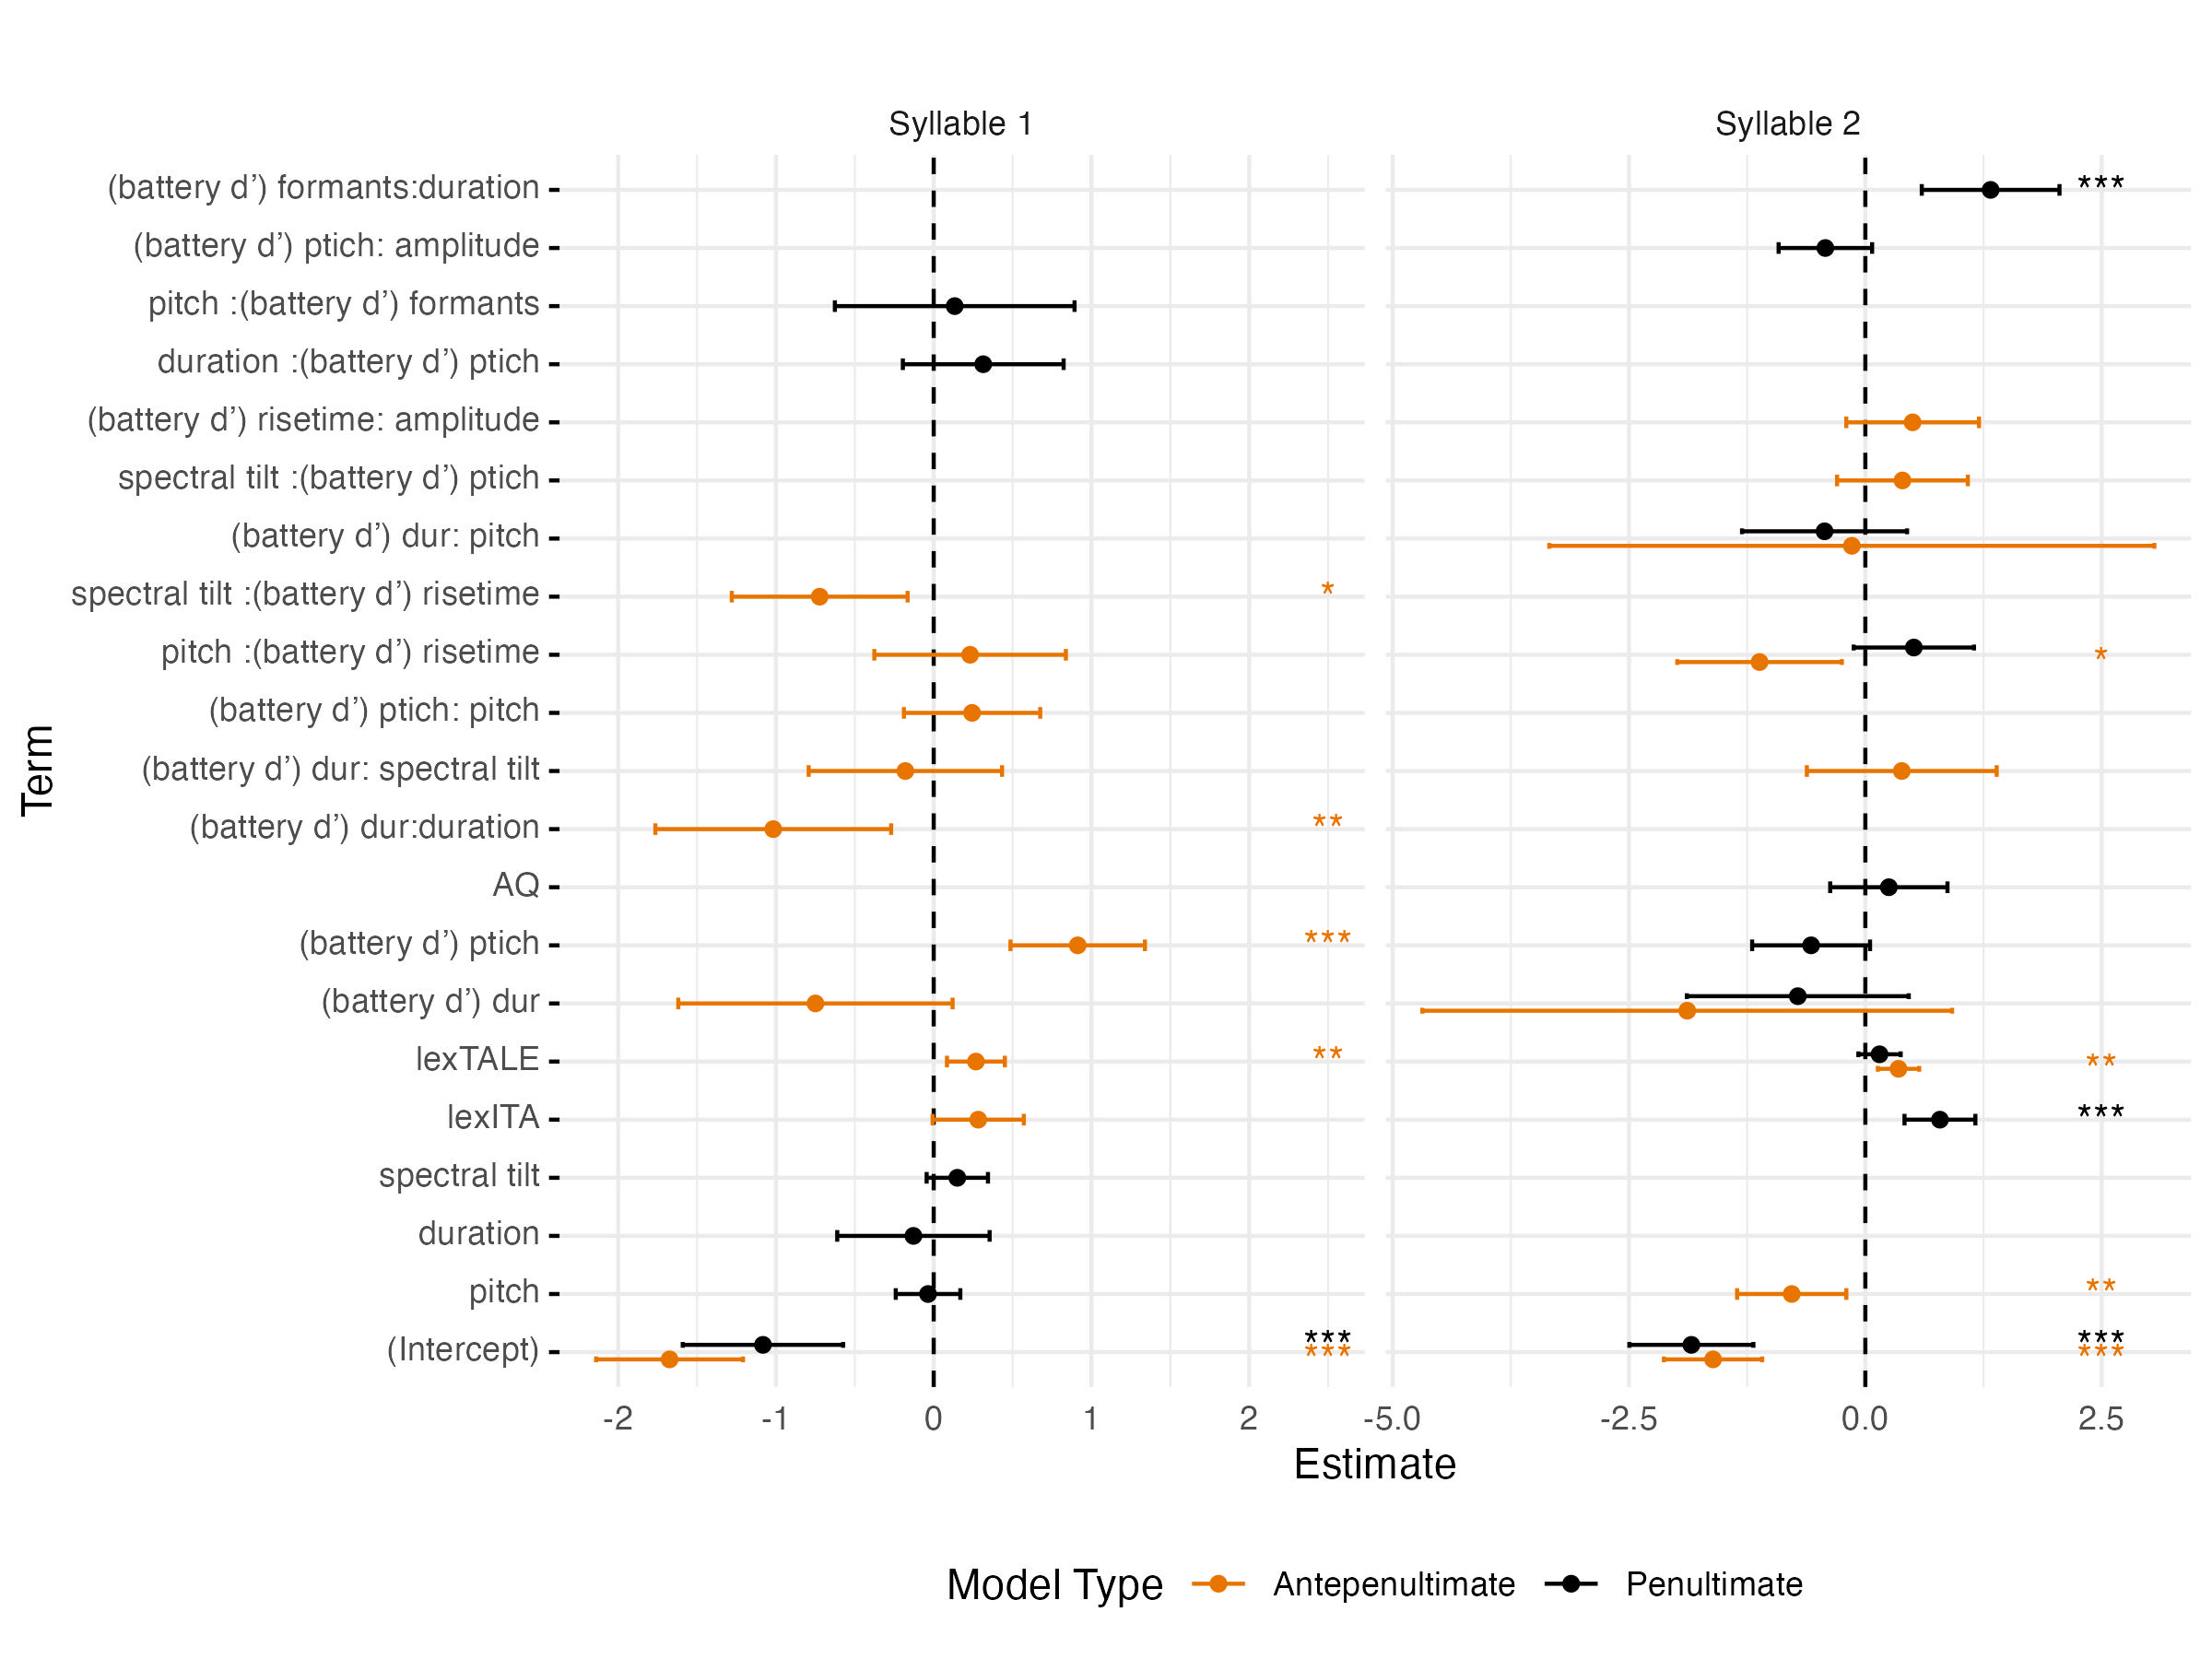
\includegraphics[width=1\linewidth]{visuals/extended_analysis.jpeg} % Adjust the width as needed
  \caption{Antepenultimate and penultimate model}
  \label{fig:extened_analysis}
\end{figure}